\textbf{Самодополнительные графы}

\begin{wrapfigure}{r}{0.3\textwidth}
    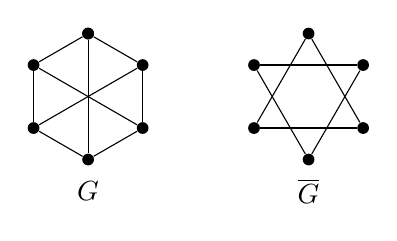
\begin{tikzpicture}[scale=0.8]
    % Первый граф (G)
    \begin{scope}[xshift=0cm]
        \foreach \angle [count=\i] in {90,150,...,450} {
            \node[circle, fill=black, inner sep=1.5pt] (v\i) at (\angle:1) {};
        }
        \foreach \i in {1,...,6} {
            \pgfmathtruncatemacro{\next}{mod(\i,6)+1}
            \draw (v\i) -- (v\next);
        }
        \draw (v1) -- (v4);
        \draw (v2) -- (v5);
        \draw (v3) -- (v6);
        \node at (0,-1.5) {$G$};
    \end{scope}
    
    % Второй граф (G с чертой)
    \begin{scope}[xshift=3.5cm]
        \foreach \angle [count=\i] in {30,90,...,389} {
            \node[circle, fill=black, inner sep=1.5pt] (w\i) at (\angle:1) {};
        }
        \foreach \i/\j in {1/3,3/5,5/1,2/4,4/6,6/2} {
            \draw (w\i) -- (w\j);
        }
        \node at (0,-1.5) {$\overline{G}$};
    \end{scope}
    \end{tikzpicture}
\end{wrapfigure}

\noindent\textbf{Дополнение графа} $\overline{G}$ (граф с теми же вершинами, но противоположными связями):
\begin{itemize}
\item Множество вершин: $V(\overline{G}) = V(G)$
\item Две вершины смежны в $\overline{G}$ $\Leftrightarrow$ несмежны в $G$
\end{itemize}

\noindent\textbf{Полный граф} $K_p$ (все вершины попарно соединены):
\begin{itemize}
\item Содержит $p$ вершин
\item Имеет $\binom{p}{2}$ рёбер
\item Является регулярным степени $p-1$
\item Частный случай: $K_3$ -- треугольник
\end{itemize}

\noindent\textbf{Вполне несвязный граф} $\overline{K_p}$ -- дополнение полного графа (регулярный граф степени 0).

\begin{figure}[h]
    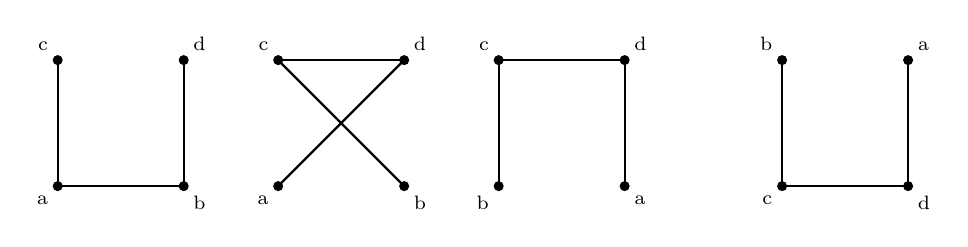
\begin{tikzpicture}[scale=0.8]
        \begin{scope}
        % Define the coordinates for the points
        \coordinate (A) at (0, 0);
        \coordinate (B) at (2, 0);
        \coordinate (C) at (0, 2);
        \coordinate (D) at (2, 2);
    
        % Draw the lines
        \draw[thick] (A) -- (B);
        \draw[thick] (A) -- (C);
        \draw[thick] (B) -- (D);
    
        % Draw the nodes and add labels
        \filldraw (A) circle (2pt) node[below left] {\scriptsize a};
        \filldraw (B) circle (2pt) node[below right] {\scriptsize b};
        \filldraw (C) circle (2pt) node[above left] {\scriptsize c};
        \filldraw (D) circle (2pt) node[above right] {\scriptsize d};
    \end{scope}
        
    
        \begin{scope}[xshift=3.5cm]
            % Define the coordinates for the points
            \coordinate (A) at (0, 0);
            \coordinate (B) at (2, 0);
            \coordinate (C) at (0, 2);
            \coordinate (D) at (2, 2);
        
            % Draw the lines
            \draw[thick] (A) -- (D);
            \draw[thick] (B) -- (C);
            \draw[thick] (C) -- (D);
        
            % Draw the nodes
            \filldraw (A) circle (2pt) node[below left] {\scriptsize a};
            \filldraw (B) circle (2pt) node[below right] {\scriptsize b};
            \filldraw (C) circle (2pt) node[above left] {\scriptsize c};
            \filldraw (D) circle (2pt) node[above right] {\scriptsize d};
            \end{scope}
    
            \begin{scope}[xshift=7cm]
                % Define the coordinates for the points
                \coordinate (A) at (0, 0);
                \coordinate (B) at (2, 0);
                \coordinate (C) at (0, 2);
                \coordinate (D) at (2, 2);
            
                % Draw the lines
                \draw[thick] (B) -- (D);
                \draw[thick] (A) -- (C);
                \draw[thick] (C) -- (D);
            
                % Draw the nodes
                \filldraw (A) circle (2pt) node[below left] {\scriptsize b};
                \filldraw (B) circle (2pt) node[below right] {\scriptsize a};
                \filldraw (C) circle (2pt) node[above left] {\scriptsize c};
                \filldraw (D) circle (2pt) node[above right] {\scriptsize d};
                \end{scope}
            
                \begin{scope}[xshift=11.5cm]
                    % Define the coordinates for the points
                    \coordinate (A) at (0, 0);
                    \coordinate (B) at (2, 0);
                    \coordinate (C) at (0, 2);
                    \coordinate (D) at (2, 2);
                
                    % Draw the lines
                    \draw[thick] (A) -- (B);
                    \draw[thick] (A) -- (C);
                    \draw[thick] (B) -- (D);
                
                    % Draw the nodes and add labels
                    \filldraw (A) circle (2pt) node[below left] {\scriptsize c};
                    \filldraw (B) circle (2pt) node[below right] {\scriptsize d};
                    \filldraw (C) circle (2pt) node[above left] {\scriptsize b};
                    \filldraw (D) circle (2pt) node[above right] {\scriptsize a};
                \end{scope}
        
    \end{tikzpicture}
    \caption{Граф - Его дополние - переворачиваем - Получили тот же граф}
\end{figure}
    